% !Mode:: "TeX:UTF-8"
% !TEX program  = xelatex

\section{问题定义与方法设计}
\label{sec:method}

\subsection{任务定义}

本文将算子选择建模为一个单步上下文老虎机任务。
设第 $t$ 个到来的实例为 $x_t$，其问题类型为 $p_t \in \{\text{TSP}, \text{CVRP}\}$。
在给定问题类型下，可选动作集合记为 $\mathcal{A}(x_t)$，
其中每个动作对应一种初始化方法。选择模型在观察实例特征后，从 $\mathcal{A}(x_t)$ 中选出动作 $a_t$，并接收该方法在当前实例上的即时反馈 $r_t(a_t)$。

因此，当前任务的决策规则可以统一写为：
\begin{equation}
  a_t = \arg\max_{a \in \mathcal{A}(x_t)} s_t(x_t, a),
  \label{eq:general-decision}
\end{equation}
其中 $s_t(x_t, a)$ 是第 $t$ 轮对动作 $a$ 的评分函数。
不同方法的差别在于这个评分函数如何定义。

\subsection{共享动作空间与可行动作约束}

TSP 与 CVRP 的可用方法并不完全相同。本文采用统一动作空间与可行动作掩码：
同时出现在两类问题中的方法（如 bq、elg、lehd）共享同一个 arm 编号，不同问题再通过 mask 过滤不可选动作。
这样既保留了方法层面的共享经验，也避免模型在某个问题上选到无效方法。
统一动作空间共包含 9 个方法，具体如表 \ref{tab:nss-arm-space} 所示。

\begin{table}[htb]
  \centering
  \caption{不同问题的可用方法}
  \label{tab:nss-arm-space}
  \begin{tabular}{clcc}
    \toprule
    arm 编号 & 方法名 & TSP 可用 & CVRP 可用 \\
    \midrule
    0 & bq~\cite{drakulic2023bqnco}         & \checkmark & \checkmark \\
    1 & elg~\cite{gao2024elg}        & \checkmark & \checkmark \\
    2 & lehd~\cite{luo2023lehd}       & \checkmark & \checkmark \\
    3 & t2t~\cite{li2023t2t}        & \checkmark & \\
    4 & t2t500~\cite{li2023t2t}     & \checkmark & \\
    5 & difusco~\cite{sun2023difusco}    & \checkmark & \\
    6 & difusco500~\cite{sun2023difusco} & \checkmark & \\
    7 & omni~\cite{zhou2023omni}       &            & \checkmark \\
    8 & mvmoe~\cite{zhou2024mvmoe}      &            & \checkmark \\
    \bottomrule
  \end{tabular}
\end{table}

\subsection{实例特征构造}

\paragraph{图编码器。}
图编码部分复用了已有工作\cite{gao2025nss}的层次化编码器。模型先用多层 attention 对节点编码，再通过 pooling 逐步下采样图结构，并聚合各层粗化图的 readout，得到最终实例表示。这里保留了 TSP 与 CVRP 各自独立的首层输入投影，因为 TSP 的节点输入是 $(x,y)$ 二维坐标，而 CVRP 还需要额外包含 demand，二者的输入维度并不相同。具体来说：
\begin{itemize}
  \item TSP 编码器接收形状为 $[B, n, 2]$ 的坐标张量；
  \item CVRP 编码器接收形状为 $[B, n+1, 3]$ 的节点张量，其中第三维为 demand。
\end{itemize}
两类编码器都输出 256 维图表示，再额外拼接一个规模特征 \texttt{scale}，形成 257 维图嵌入。

\paragraph{手工特征。}
手工特征延续了参考工作\cite{gao2025nss}的统计思路，主要包括节点分布的离散程度、质心位置、半径、最近邻距离波动、聚类相关统计量，以及 CVRP 的需求均值与需求标准差，总维度为 11。

\paragraph{问题类型编码。}
问题类型 one-hot 是二维向量：TSP 对应 $[1,0]$，CVRP 对应 $[0,1]$。

\paragraph{实例特征}
实例特征由三部分拼接得到：
\begin{equation}
  c(x) = [g(x), m(x), o(p)],
  \label{eq:context}
\end{equation}
其中 $g(x)$ 表示图编码结果，$m(x)$ 表示手工统计特征，$o(p)$ 表示问题类型 one-hot。
因此，实例编码维度为：
\begin{equation}
  \dim(c(x)) = 257 + 11 + 2 = 270.
\end{equation}

\subsection{reward 设计}

不同问题的原始 cost 量级差异较大，
若直接将绝对 cost 用作训练 reward，数值尺度会明显不稳定。
本文采用实例内排名 reward，把成本最小化转成排名最优化：
\begin{equation}
  r(x, a) = 1 - \frac{\operatorname{rank}(x, a) - 1}{|\mathcal{A}(x)| - 1},
  \label{eq:rank-reward}
\end{equation}
其中 $\operatorname{rank}(x, a)=1$ 表示方法 $a$ 在实例 $x$ 上 cost 最低。于是最优方法的 reward 为 1，最差方法的 reward 为 0，其余方法线性插值。

需要指出的是，排名 reward 与最终 mean length 目标之间并不完全一致。
排名只保留了方法之间的序关系，丢弃了绝对成本差距的信息：
当某实例上所有方法的 cost 差异很小时，排名 reward 的区分度与对最终 cost 的贡献不成比例。
本文在实验部分（第 \ref{sec:results}节）将进一步讨论这一偏差的影响。

\paragraph{训练与评估协议。}
本文的训练数据来自离线阶段：对每个训练实例，预先运行所有候选方法并记录各自的 cost，从而获得全信息的 reward 矩阵。
但在训练过程中，模型按在线老虎机协议运行——每次只观察被选动作的 reward，不使用未选动作的信息。
这一设定模拟了实际部署场景：历史结果可离线批量生成，但在线阶段只能获得部分反馈。

\subsection{Neural-LinUCB}

Neural-LinUCB 的核心思想，是把深度表征学习与浅层探索分开处理：
神经网络负责学习实例表示，UCB 探索则限制在低维线性空间内\cite{xu2022neurallinucb}。
$x$ 表示一个实例，$a$ 表示一个候选初始化方法，
$r(x,a)$ 表示在实例 $x$ 上选择方法 $a$ 后的期望 reward。
其基本形式为
\begin{equation}
  r(x,a)=\theta^\top \phi(x,a),
\end{equation}
其中 $\phi(x,a)$ 是实例--动作对的深度表征，$\theta$ 是作用在该表征上的线性参数。
我们用 $\psi$ 表示共享表示层的全部参数，包括图编码器、特征融合层和动作条件 MLP 的参数。
因此，深度表征写为
\begin{equation}
  \phi(x, a) = f_\psi([c(x), e(a)]),
  \label{eq:phi}
\end{equation}
其中 $c(x) \in \mathbb{R}^{270}$ 是实例上下文，$e(a) \in \mathbb{R}^{16}$ 是方法 $a$ 的可学习嵌入，$[\cdot,\cdot]$ 表示向量拼接，$f_\psi(\cdot)$ 为两层 MLP。
于是，拼接后的输入维度为 $270 + 16 = 286$，最终输出
\[
  \phi(x,a) \in \mathbb{R}^{64}.
\]
这意味着所有候选方法都会被映射到同一个 64 维动作条件表示空间，再由线性 UCB 头完成打分。
整体架构见图~\ref{fig:method-architecture}。

\begin{figure}[htb]
  \centering
  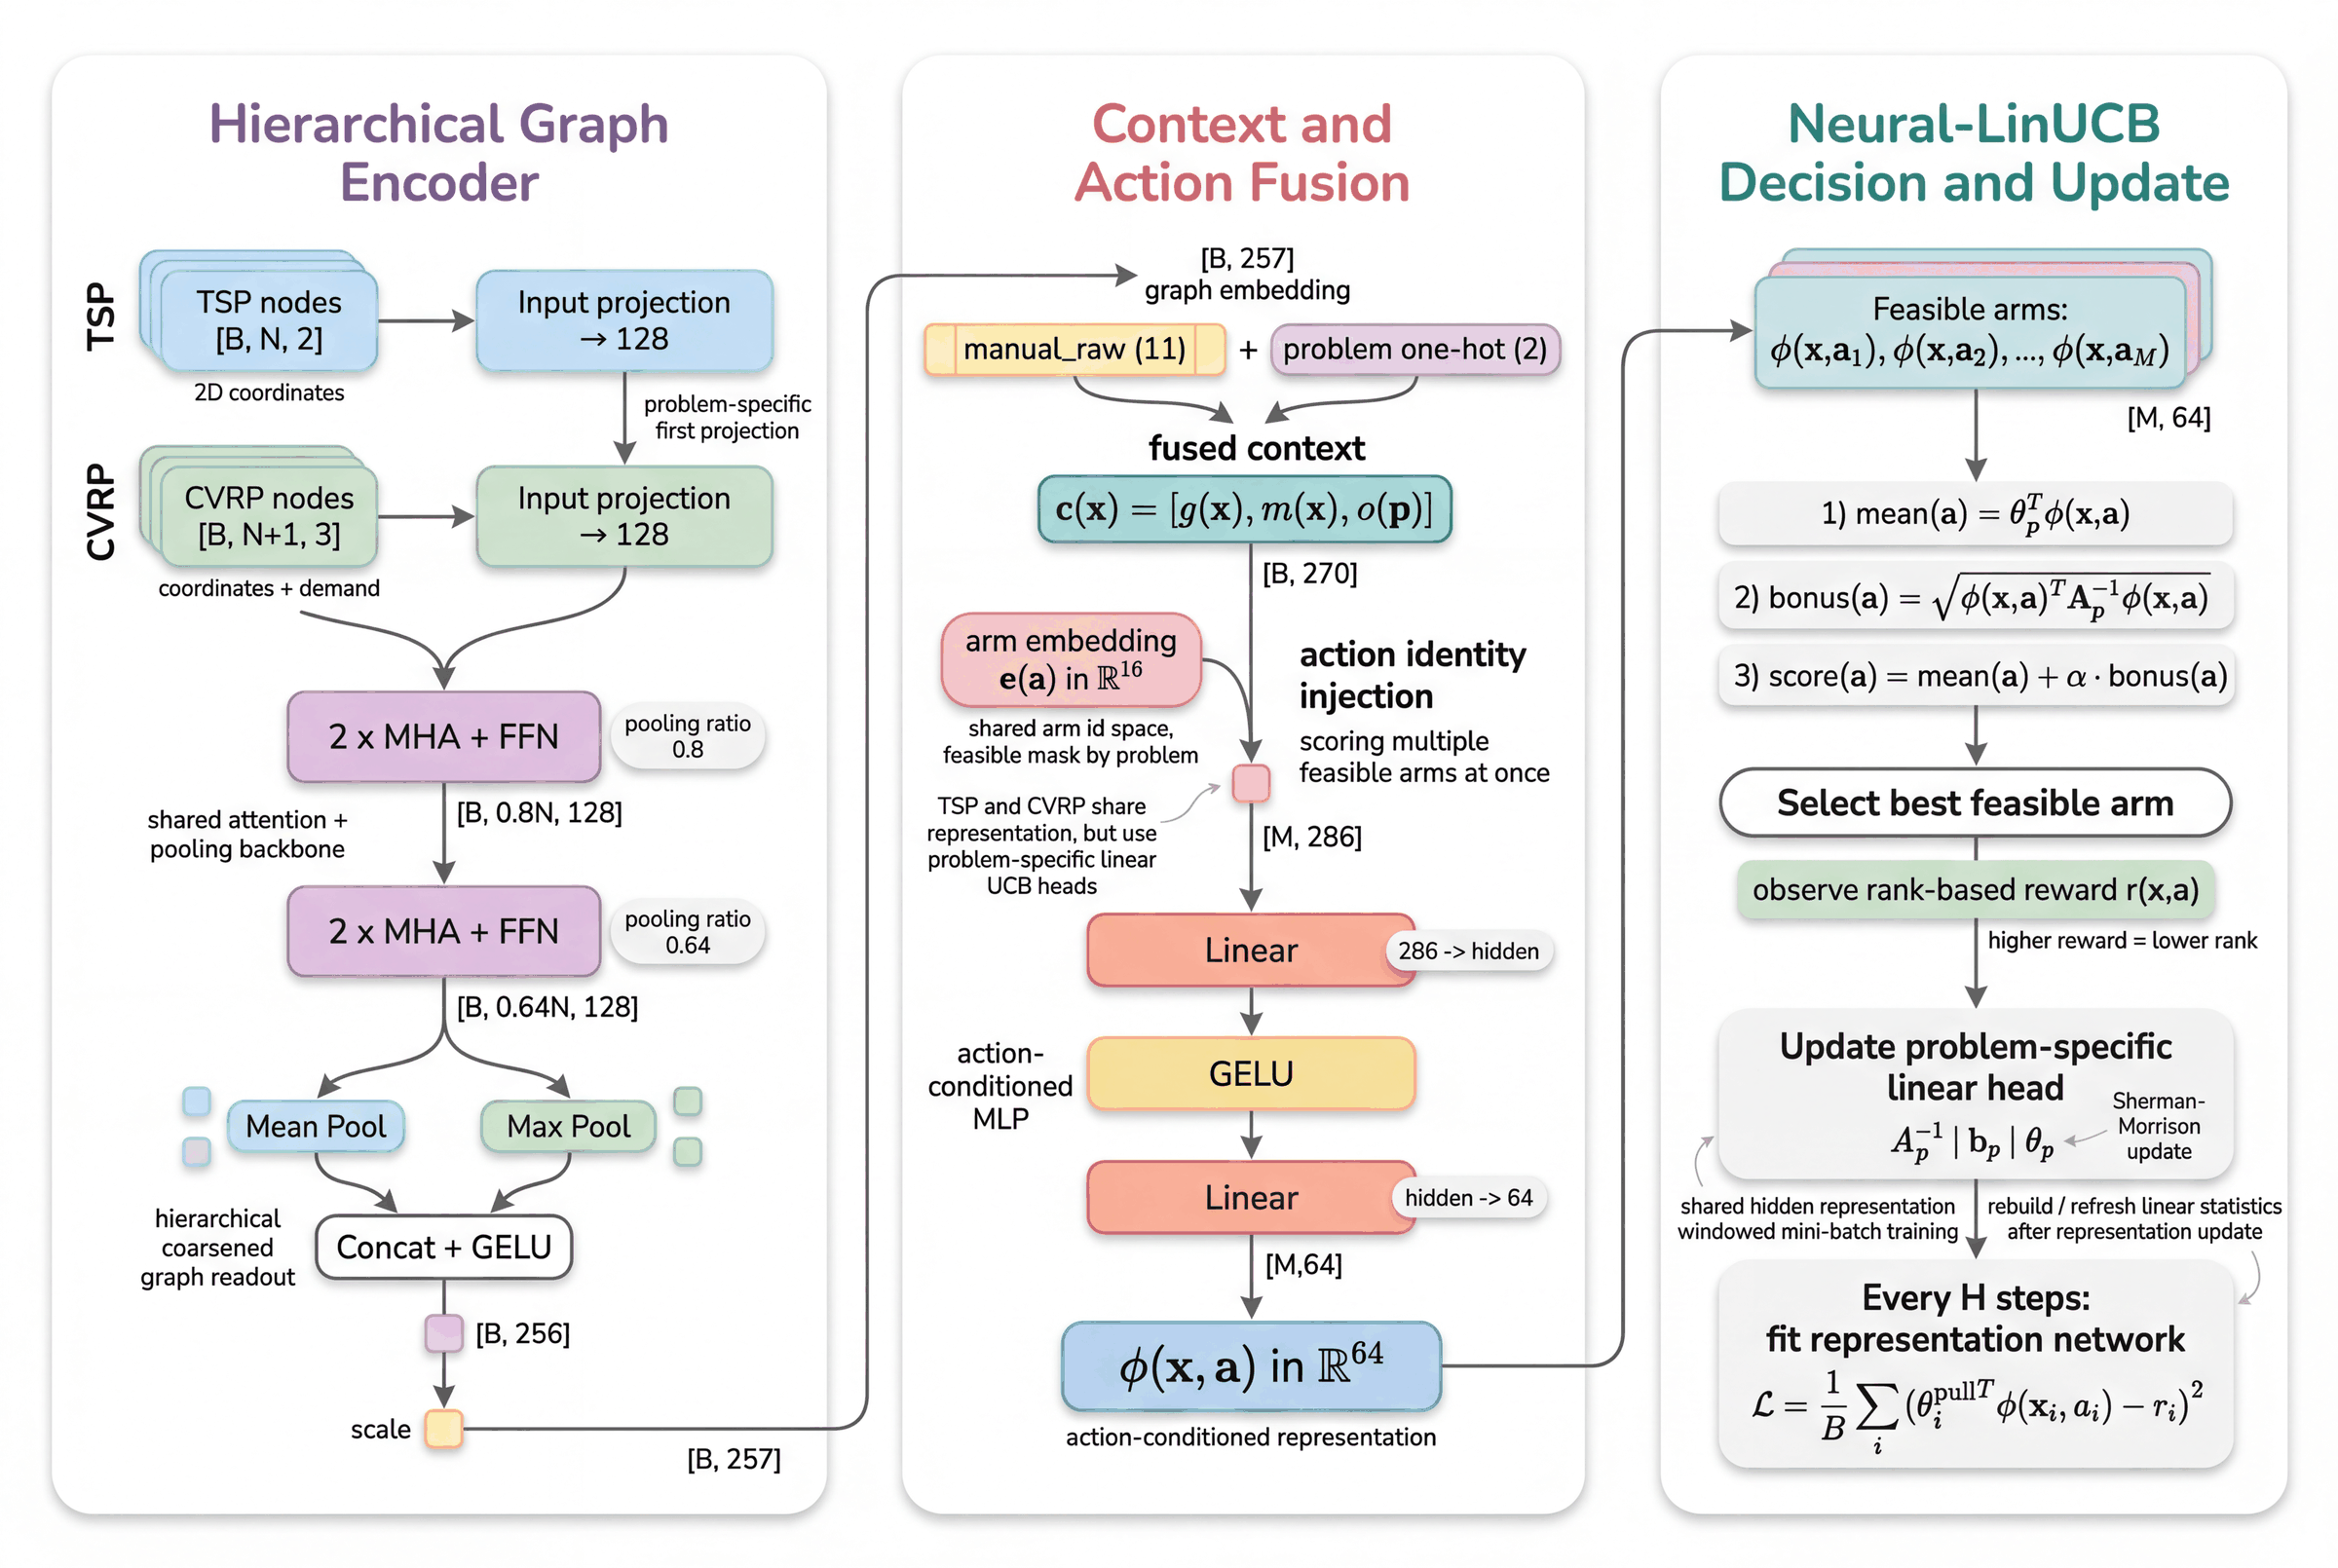
\includegraphics[width=\textwidth]{figures/research/figure-07-method-architecture.png}
  \caption{本文方法的整体架构。模型首先对实例进行问题相关的图编码，并与手工特征和问题类型编码融合为上下文表示；随后结合方法嵌入构造动作条件表示 $\phi(x,a)$；最后通过按问题拆分的线性 UCB 头完成可行动作筛选、评分、选择以及在线更新。}
  \label{fig:method-architecture}
\end{figure}

给定问题类型 $p_t$ 对应的线性头参数 $(A_{p_t,t}^{-1}, b_{p_t,t}, \theta_{p_t,t})$，动作评分函数写为：
\begin{equation}
  s_t(x_t, a) =
  \theta_{p_t,t}^{\top} \phi(x_t, a)
  + \alpha \sqrt{\phi(x_t, a)^{\top} A_{p_t,t}^{-1} \phi(x_t, a)},
  \label{eq:neural-linucb-score}
\end{equation}
各个量的含义如下：
$\theta_{p_t,t} \in \mathbb{R}^{64}$ 是问题 $p_t$ 在时刻 $t$ 的线性头参数，
$A_{p_t,t}^{-1} \in \mathbb{R}^{64\times 64}$ 是该问题对应协方差矩阵的逆，
$b_{p_t,t} \in \mathbb{R}^{64}$ 是 reward 加权的特征累积向量。
式 \eqref{eq:neural-linucb-score} 的第一项
$\theta_{p_t,t}^{\top} \phi(x_t, a)$
是利用项（exploitation term），表示当前线性头对动作 $a$ 的 reward 预测；
第二项
$\sqrt{\phi(x_t, a)^{\top} A_{p_t,t}^{-1} \phi(x_t, a)}$
是探索项（exploration term），衡量动作 $a$ 在当前线性模型下的不确定性；
$\alpha$ 为探索强度，用来调节这两项之间的权衡。
若某个动作在当前问题上的历史观测较少，其探索项通常更大，因此更容易被选中。
当前实现采用共享表示层、按问题拆分的线性 UCB 头，
即 TSP 与 CVRP 共享同一套深度表征，但分别维护各自的线性统计量和不确定性估计。

\subsection{在线更新与表示层训练}

当选择器在第 $t$ 轮选中动作 $a_t$ 并观察到 reward $r_t$ 后，线性头按标准 LinUCB 形式增量更新。
在线性 UCB 中，矩阵 $A_{p,t}$ 为该问题在表示空间中的二阶统计量，
向量 $b_{p,t}$ 累积了 reward 加权后的特征。
如果每一步都重新计算 $A_{p,t}^{-1}$，代价会较高，因此这里直接维护逆矩阵，并通过 Sherman--Morrison 公式更新：
\begin{equation}
  A_{p,t}^{-1}
  \leftarrow
  A_{p,t-1}^{-1}
  -
  \frac{A_{p,t-1}^{-1}\phi_t \phi_t^{\top} A_{p,t-1}^{-1}}
  {1 + \phi_t^{\top} A_{p,t-1}^{-1} \phi_t},
\end{equation}
随后更新
\begin{equation}
  b_{p,t} \leftarrow b_{p,t-1} + r_t \phi_t,
  \qquad
  \theta_{p,t} \leftarrow A_{p,t}^{-1} b_{p,t}.
\end{equation}
这一步的作用是把新观测到的 $(\phi_t, r_t)$ 纳入当前问题的线性头：
$b_{p,t}$ 吸收 reward 信号，
$\theta_{p,t}$ 则给出该问题在 64 维表示空间中的线性 reward 估计。

表示层训练采用周期性、窗口化的小批量更新。
设最近一个表示层窗口中的历史记录为
\[
  \mathcal{D}_{\mathrm{rep}}
  =
  \{(x_i, a_i, r_i, \theta_i^{\text{pull}})\}_{i=1}^{B},
\]
其中 $B$ 为当前小批量大小，$\theta_i^{\text{pull}}$ 表示第 $i$ 条样本在被选中时缓存下来的线性头参数。
每隔若干 step，从该窗口中抽取一个小批量，用当前网络输出的 $\phi(x_i, a_i)$ 与对应的 $\theta_i^{\text{pull}}$ 做内积，拟合真实 reward：
\begin{equation}
  \mathcal{L}(\psi)
  =
  \frac{1}{B}
  \sum_{i=1}^{B}
  \left(
    {\theta_i^{\text{pull}}}^{\top}\phi(x_i, a_i)-r_i
  \right)^2.
  \label{eq:representation-loss}
\end{equation}
这里，
${\theta_i^{\text{pull}}}^{\top}\phi(x_i, a_i)$
是当前表示层在第 $i$ 条历史样本上的预测值，
$r_i$ 是该样本真实观测到的 reward。

为了更清楚地展示选择、更新和表示层重训练之间的关系，
算法~\ref{alg:neural-linucb-online} 总结了本文方法在一次完整在线遍历中的主流程。

\begin{algorithm}[htb]
  \caption{算子选择的 Problem-Specific Neural-LinUCB 在线流程}
  \label{alg:neural-linucb-online}
  \small
  \begin{algorithmic}[1]
    \Require 实例序列 $\{(x_t, p_t)\}_{t=1}^T$，共享表示网络 $\phi(x,a)$，可行动作集合 $\mathcal{A}(x_t)$，探索系数 $\alpha$，表示层更新周期 $H$
    \State 对每个问题 $p \in \{\mathrm{TSP}, \mathrm{CVRP}\}$ 初始化 $(A_p^{-1}, b_p, \theta_p)$
    \State 初始化表示层缓存 $\mathcal{D}_{\mathrm{rep}}$ 与线性头缓存 $\mathcal{D}_{\mathrm{lin}}$
    \For{$t = 1, 2, \dots, T$}
      \State 接收实例 $x_t$ 与问题类型 $p_t$
      \State 构造当前实例的可行动作集合 $\mathcal{A}(x_t)$
      \For{each $a \in \mathcal{A}(x_t)$}
        \State 编码 $\phi_t(a) \gets \phi(x_t, a)$
        \State 计算分数 $s_t(a) \gets \theta_{p_t}^{\top}\phi_t(a) + \alpha \sqrt{\phi_t(a)^{\top} A_{p_t}^{-1}\phi_t(a)}$
      \EndFor
      \State 选择动作 $a_t \gets \arg\max_{a \in \mathcal{A}(x_t)} s_t(a)$
      \State 观察即时反馈 $r_t$
      \State 将 $(x_t, a_t, r_t, \theta_{p_t})$ 存入 $\mathcal{D}_{\mathrm{rep}}$，将 $(x_t, a_t, r_t)$ 存入 $\mathcal{D}_{\mathrm{lin}}$
      \State 取 $\phi_t \gets \phi(x_t, a_t)$
      \State 用 Sherman--Morrison 公式更新 $A_{p_t}^{-1}$
      \State 更新 $b_{p_t} \gets b_{p_t} + r_t \phi_t$，$\theta_{p_t} \gets A_{p_t}^{-1} b_{p_t}$
      \If{$t \bmod H = 0$}
        \State 在最近的表示层窗口上拟合 $\mathcal{L}(\psi)$
        \State 用线性头窗口重新构建各问题的 $(A_p^{-1}, b_p, \theta_p)$
      \EndIf
    \EndFor
  \end{algorithmic}
\end{algorithm}

这一设计保留了 Neural-LinUCB 深度表征与浅层探索解耦的基本思路，同时结合当前任务做了两项改动：
\begin{itemize}
  \item 采用最近窗口而非全部历史来训练表示层，以控制训练时间；
  \item 在表示层训练后，使用线性头窗口重新构建 $A^{-1}$、$b$ 和 $\theta$，避免旧的线性统计量与新的特征空间不一致。
\end{itemize}
